\chapter{Datasets}
\label{chap:cpv:data}

This analysis uses all data collected in 2011 and 2012.
As the beam conditions changed between the two years, from \sqrtseq{7} to 
\SI{8}{\TeV}, the analysis is performed separately on the two sub-samples.
The sub-samples are further split into magnet up and magnet down datasets, as 
the particle detection asymmetries change with the magnet 
polarity~\cite{Vesterinen:1642153}.
The individual measurements made using these sub-samples are later combined in 
an average.
The total integrated luminosity is \totlumi, the breakdown of which for the 
different running conditions is given in \cref{tab:cpv:data:luminosity}.
This \lcnamecref{chap:cpv:data} will describe the generalities of the data, 
such as the processing workflow and application of calibrations, as well as the 
simulated \ac{MC} data that will be used.

The data are processed through the offline reconstruction and the stripping, as 
described in \cref{chap:intro:lhcb:offline}.
Two stripping lines select the \LcTopKK\ and \LcToppipi\ decays of interest in 
association with a muon candidate, and a $\PLambdac\Pmuon$ vertex is formed and 
treated as a \PLambdab.
The candidates passing the stripping selections are required to have been used 
in specific trigger decisions.
As combinatorial background is the dominant component in the data at this 
stage, as shown in \cref{fig:cpv:data:mass}, candidates passing the stripping 
and trigger requirements are further filtered offline.
Details of the trigger, stripping, and offline selection will be given in 
\cref{chap:cpv:selection}.

\begin{figure}
  \begin{subfigure}[b]{0.5\textwidth}
    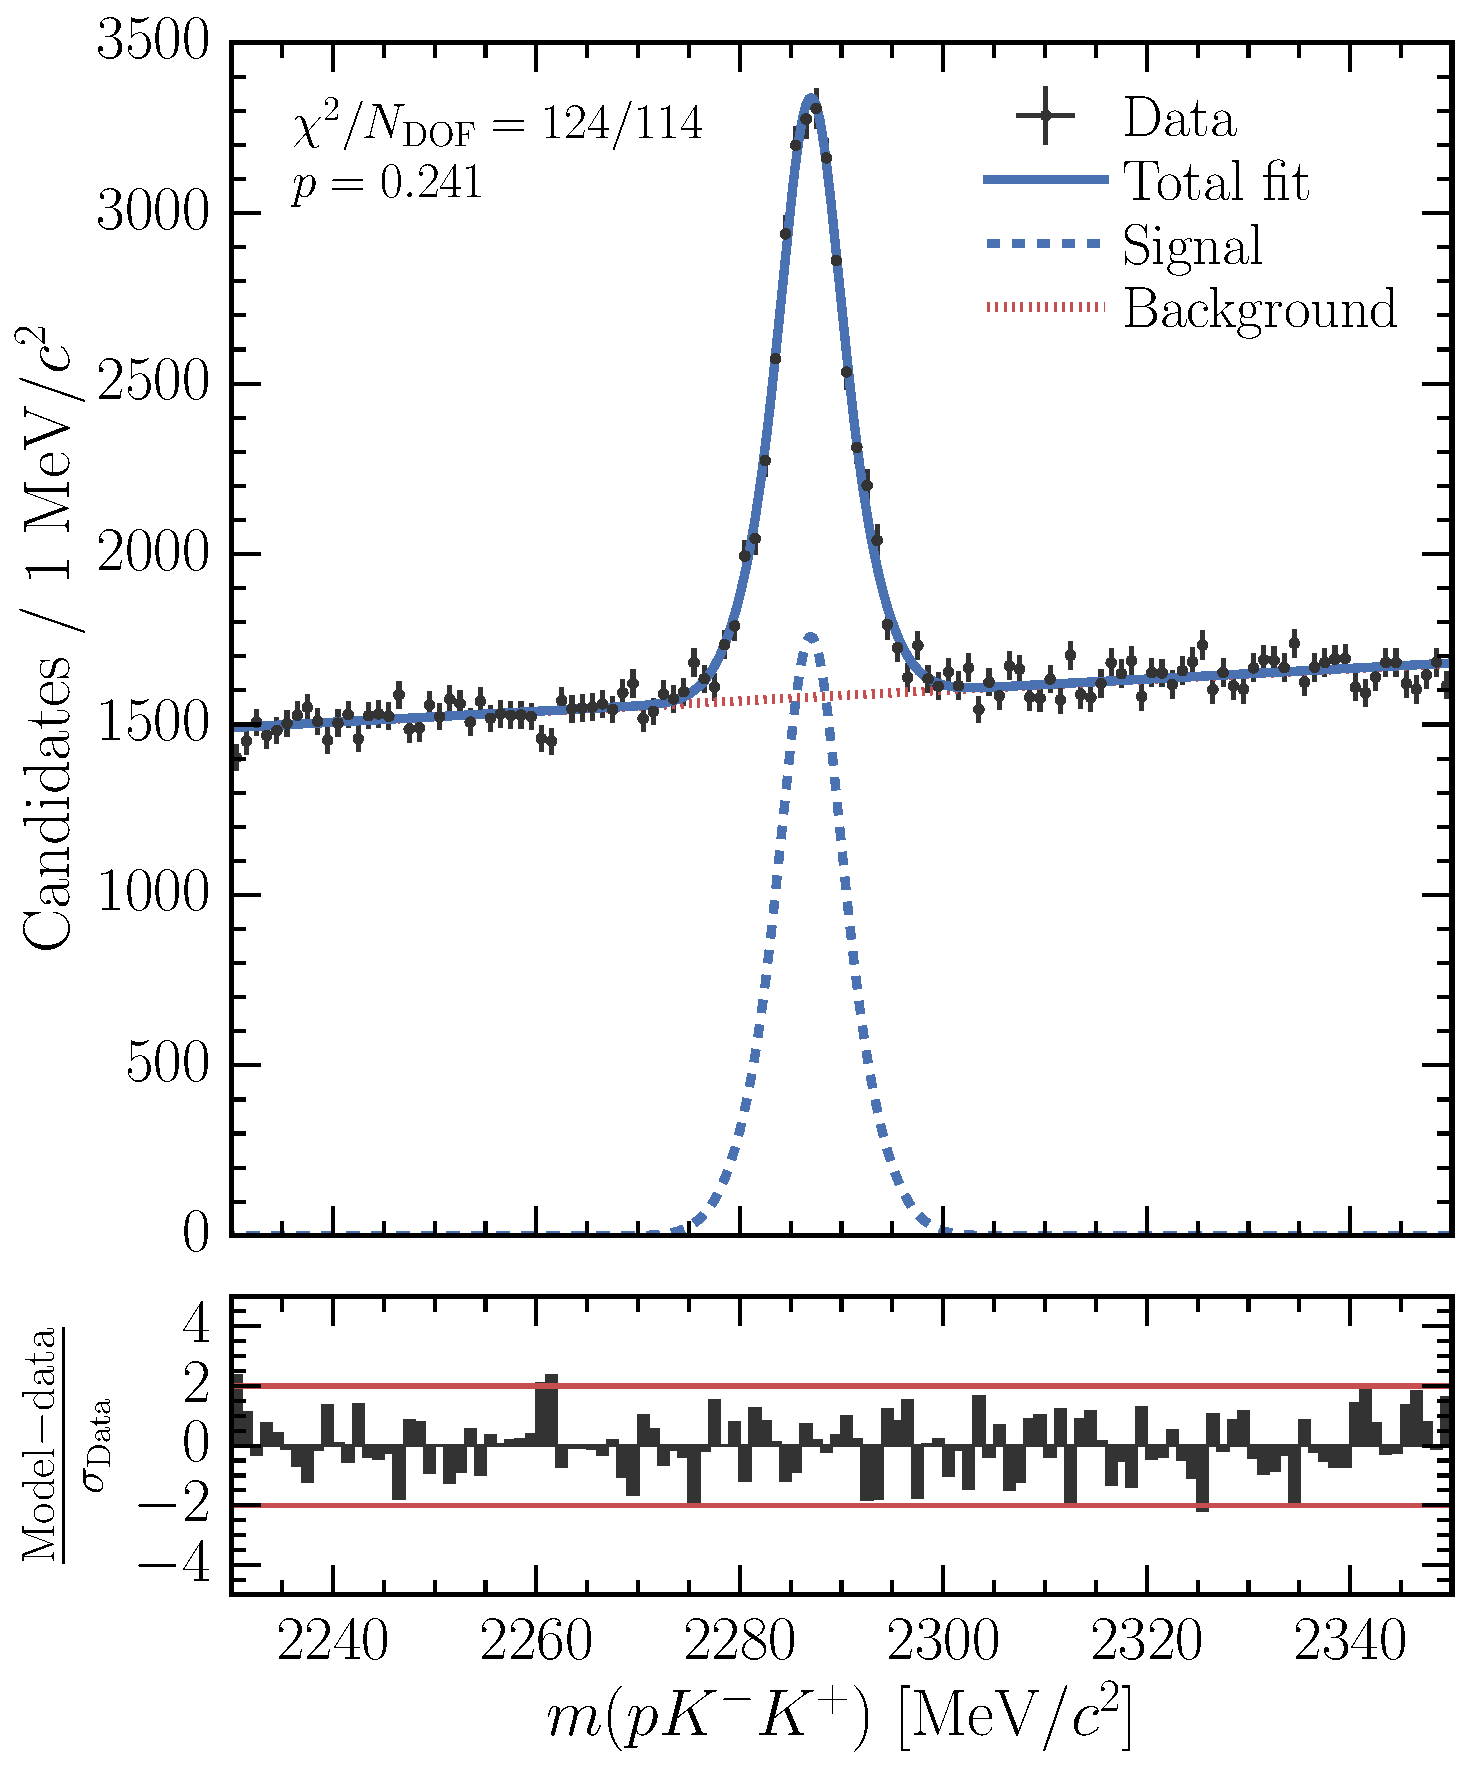
\includegraphics[width=\textwidth]{cpv/data/fits-stripping_trigger-selection_unweighted_no-simultaneous/LcTopKK_2012_MagDown_fit.pdf}
    \caption{\pKK}
    \label{fig:cpv:data:mass:pKK}
  \end{subfigure}
  \begin{subfigure}[b]{0.5\textwidth}
    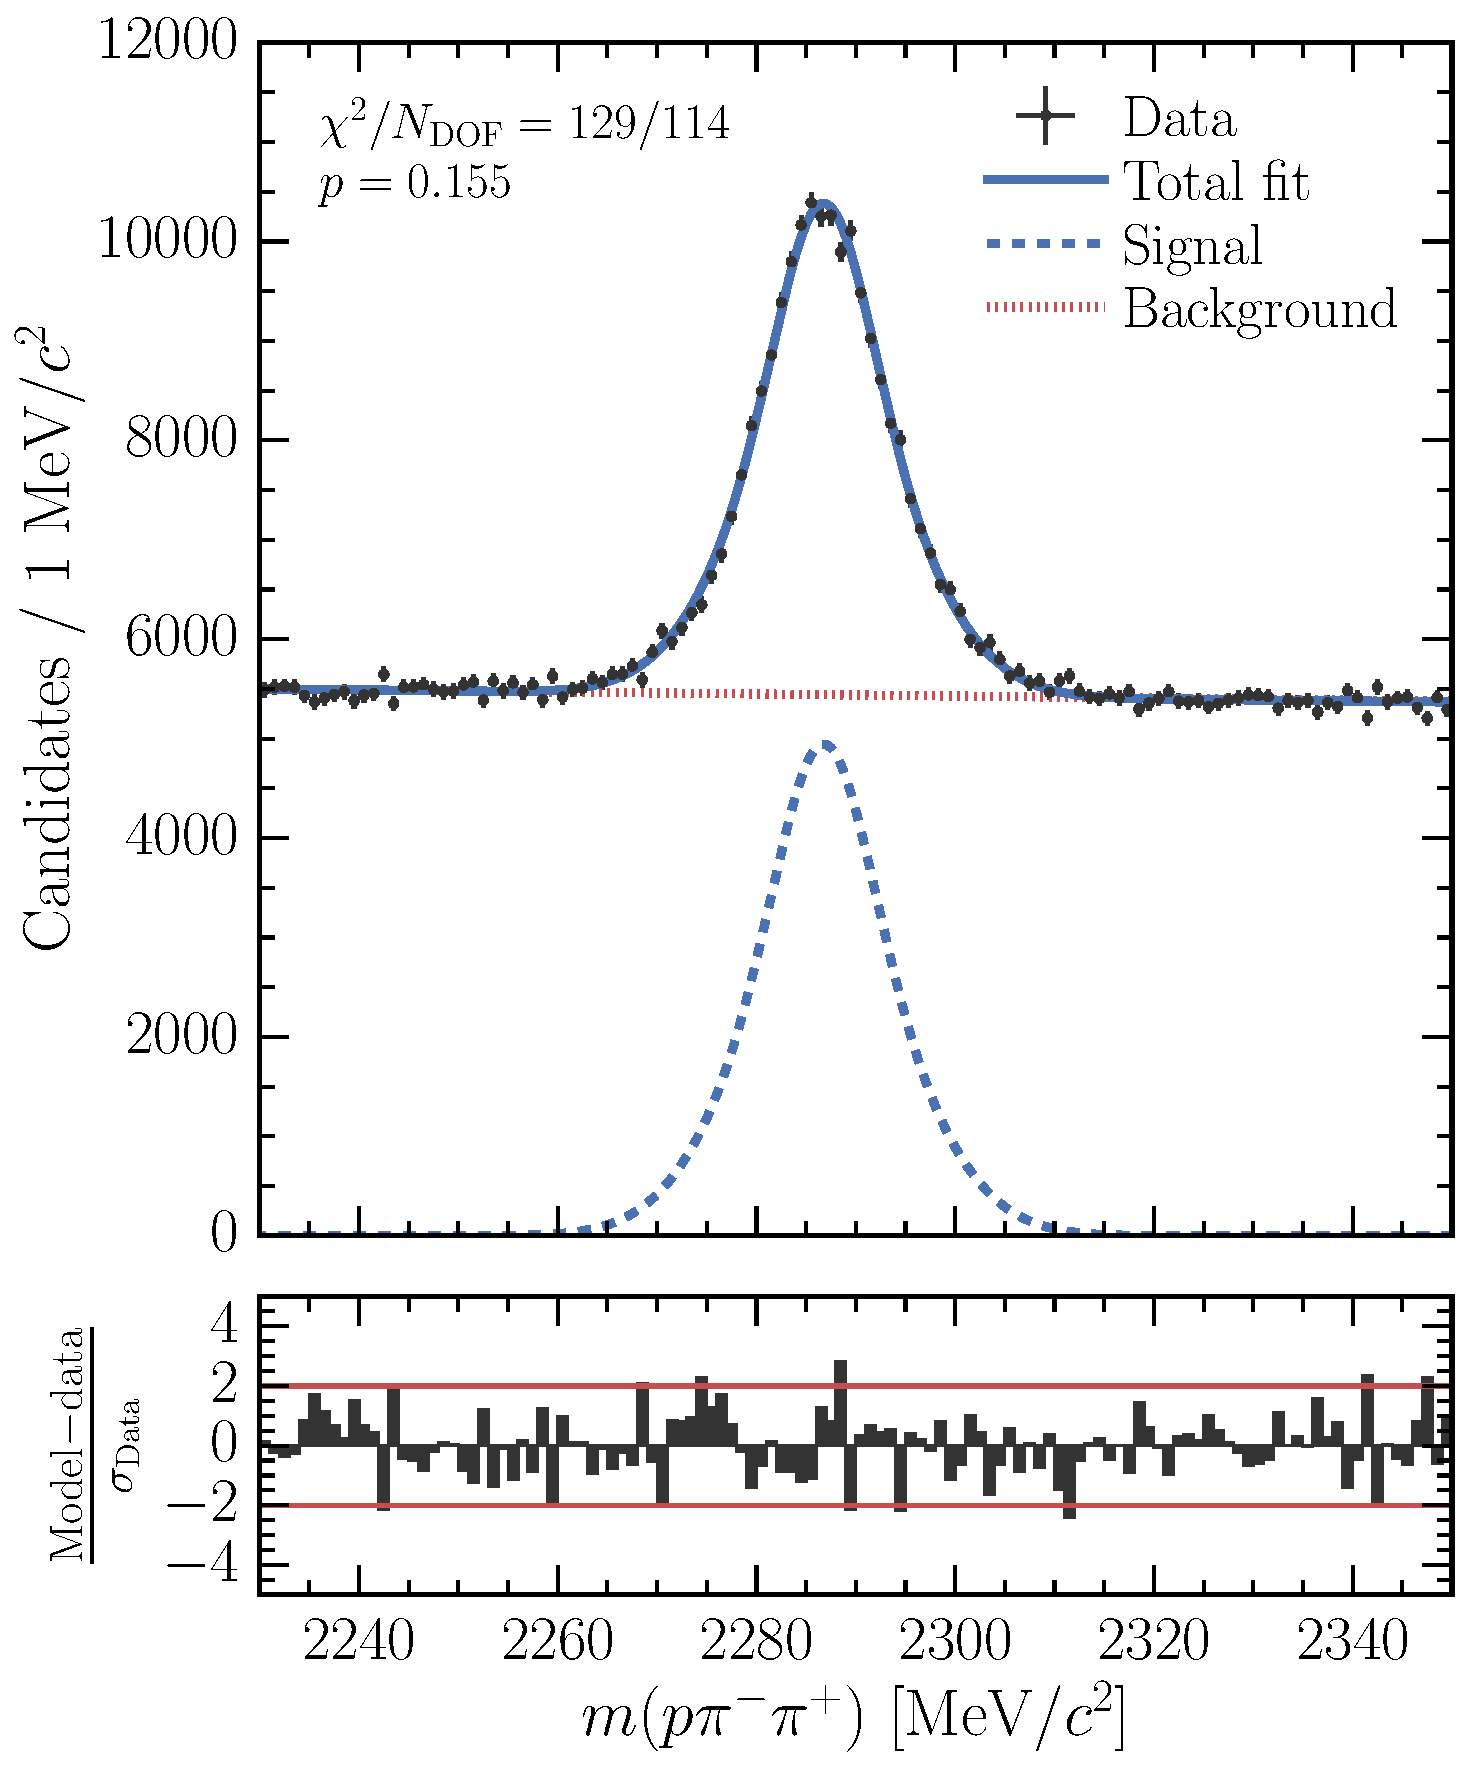
\includegraphics[width=\textwidth]{cpv/data/fits-stripping_trigger-selection_unweighted_no-simultaneous/LcToppipi_2012_MagDown_fit.pdf}
    \caption{\ppipi}
    \label{fig:cpv:data:mass:ppipi}
  \end{subfigure}
  \caption{%
    Fits to the \PLambdac\ mass spectrum in the 2012 magnet down dataset for 
    \pKK\ (\subref*{fig:cpv:data:mass:pKK}) and \ppipi\ 
    (\subref*{fig:cpv:data:mass:ppipi}).
    Only the stripping and trigger selection is applied.
    The fit that is overlaid is described in \cref{chap:cpv:prelim_fits}.
  }
  \label{fig:cpv:data:mass}
\end{figure}

To improve the \PLambdac\ mass resolution in the datasets, and the consistency 
between them, two algorithms are run on the data offline.
The first of these is the momentum scale calibration.
This corrects track momentum by a linear factor $\alpha$, which varies with 
running conditions and is found by comparing mass measurements made with 
\JpsiTomumu\ and \decay{\PBplus}{\PJpsi\PKplus} decays to the corresponding 
world averages~\cite{Aaij:2014jba}.
The second algorithm is \decaytreefitter~\cite{Hulsbergen:2005pu}.
This fits the entire \LbToLcmuX-with-\LcTophh\ decay chain in a single step, 
rather than the back-to-front (or leaf-by-leaf) reconstruction used in the 
stripping.
The advantage of such a method is that all the information known about the 
decay can influence the fit parameters, whereas the stripping reconstruction 
can only propagate information in one direction.
Such a global treatment of information is particularly useful when applying 
constraints in the fit, such as requiring the mass of a vertex combination to 
be exactly some value, or that the head of the decay originated from the 
\ac{PV}.
In this analysis, \decaytreefitter\ is applied to the \PLambdab\ decay with the 
constraint that the \phh\ vertex has the nominal \PLambdac\ mass of 
\SI{2286}{\MeVcc}~\cite{PDG2014}.
This improves the resolution of the \PLambdac\ phase space variables, and 
restricts the phase space to physical values.
Unless stated otherwise, kinematic quantities used in this analysis are those 
computed by the \decaytreefitter\ algorithm, with the notable exceptions of the 
quantities used in the trigger and stripping selections, and the \phh\ 
invariant mass entering the mass fit.

\section{Monte Carlo}
\label{chap:cpv:data:mc}

The only information made available for offline analysis is that passing the 
stripping.
Simulated data are used to infer properties of the data before that stage.
There are three different sets of Monte Carlo~(MC) data that are used in this 
analysis.

\subsection{Full detector simulation}
\label{chap:cpv:data:mc:full}

The full \lhcb\ Monte Carlo is used to obtain distributions of the phase space 
variables after the \lhcb\ acceptance, stripping, trigger, and offline 
requirements.
The general procedure of the \lhcb\ \ac{MC} generation is described in 
\cref{chap:prod:data:mc}, and the acceptance requirements are identical to 
those given in \cref{eqn:prod:data:lhcb_acceptance}.

The samples contain around \num{2.5e6} generated \PLambdab\ decays per 
\PLambdac\ final state per magnet polarity, simulated using the most 
representative data-taking conditions for 2012.
These conditions correspond to an average number of \pp\ interactions per bunch 
crossing of $\nu = 2.5$, a beam energy of \SI{4}{\TeV}, and a trigger 
configuration representative of the average trigger conditions used in 2012.
Each \PLambdab\ is forced to decay to the $\PLambdac\Pmuon\APnum$ final state, 
and the \PLambdac\ is forced to decay to the appropriate \phh\ final state with 
no intermediate resonances.
The simulated data are reconstructed with the same reconstruction software as 
the real data, and are then passed through a near-identical version of the 
stripping, with the only difference being the omission of any \ac{PID} 
selection, as the related variables are known to be poorly modelled in the 
\ac{MC}.
The \decaytreefitter\ algorithm is run on the candidates passing the stripping, 
but the momentum scale calibration is not applied as the conditions in the 
\ac{MC} are stable.

\subsection{Generator-level simulation}
\label{chap:cpv:data:mc:gen}

The Monte Carlo samples described in \cref{chap:cpv:data:mc:full} have the 
\lhcb\ acceptance requirements imposed upon them, as defined in 
\cref{eqn:prod:data:lhcb_acceptance}.
These requirements do not necessarily have a flat efficiency across the 
\LcTophh\ phase space, and so additional samples are required to study these 
effects.
A sample of \num{5e5} \LbToLcmunu\ decays are generated for each \LcTophh\ mode 
for each 2012 magnet polarity.
These samples are not propagated through the detector simulation, and so only 
generator-level, or `truth level', information is available.

\begin{table}
  \centering
  \caption{%
    Integrated luminosity for each data sample used in the analysis.
  }
  \label{tab:cpv:data:luminosity}
  \begin{tabular}{ccS}
  \toprule
  Year & Polarity & {Integrated luminosity (\si{\per\pico\barn})} \\
  \midrule
  2011 & Up       & 422 \pm 7                                   \\
  2011 & Down     & 564 \pm 10                                  \\
  2012 & Up       & 1001 \pm 12                                 \\
  2012 & Down     & 993 \pm 12                                  \\
  \bottomrule
\end{tabular}

\end{table}
